\documentclass[border=10pt]{standalone}

\usepackage{tikz}
\usepackage{tikzsymbols}
\usetikzlibrary{calc,patterns,shapes.geometric}

\def\centerarc[#1](#2)(#3:#4:#5){\draw[#1] ($(#2)+({#5*cos(#3)},{#5*sin(#3)})$) arc (#3:#4:#5);}

\begin{document}
	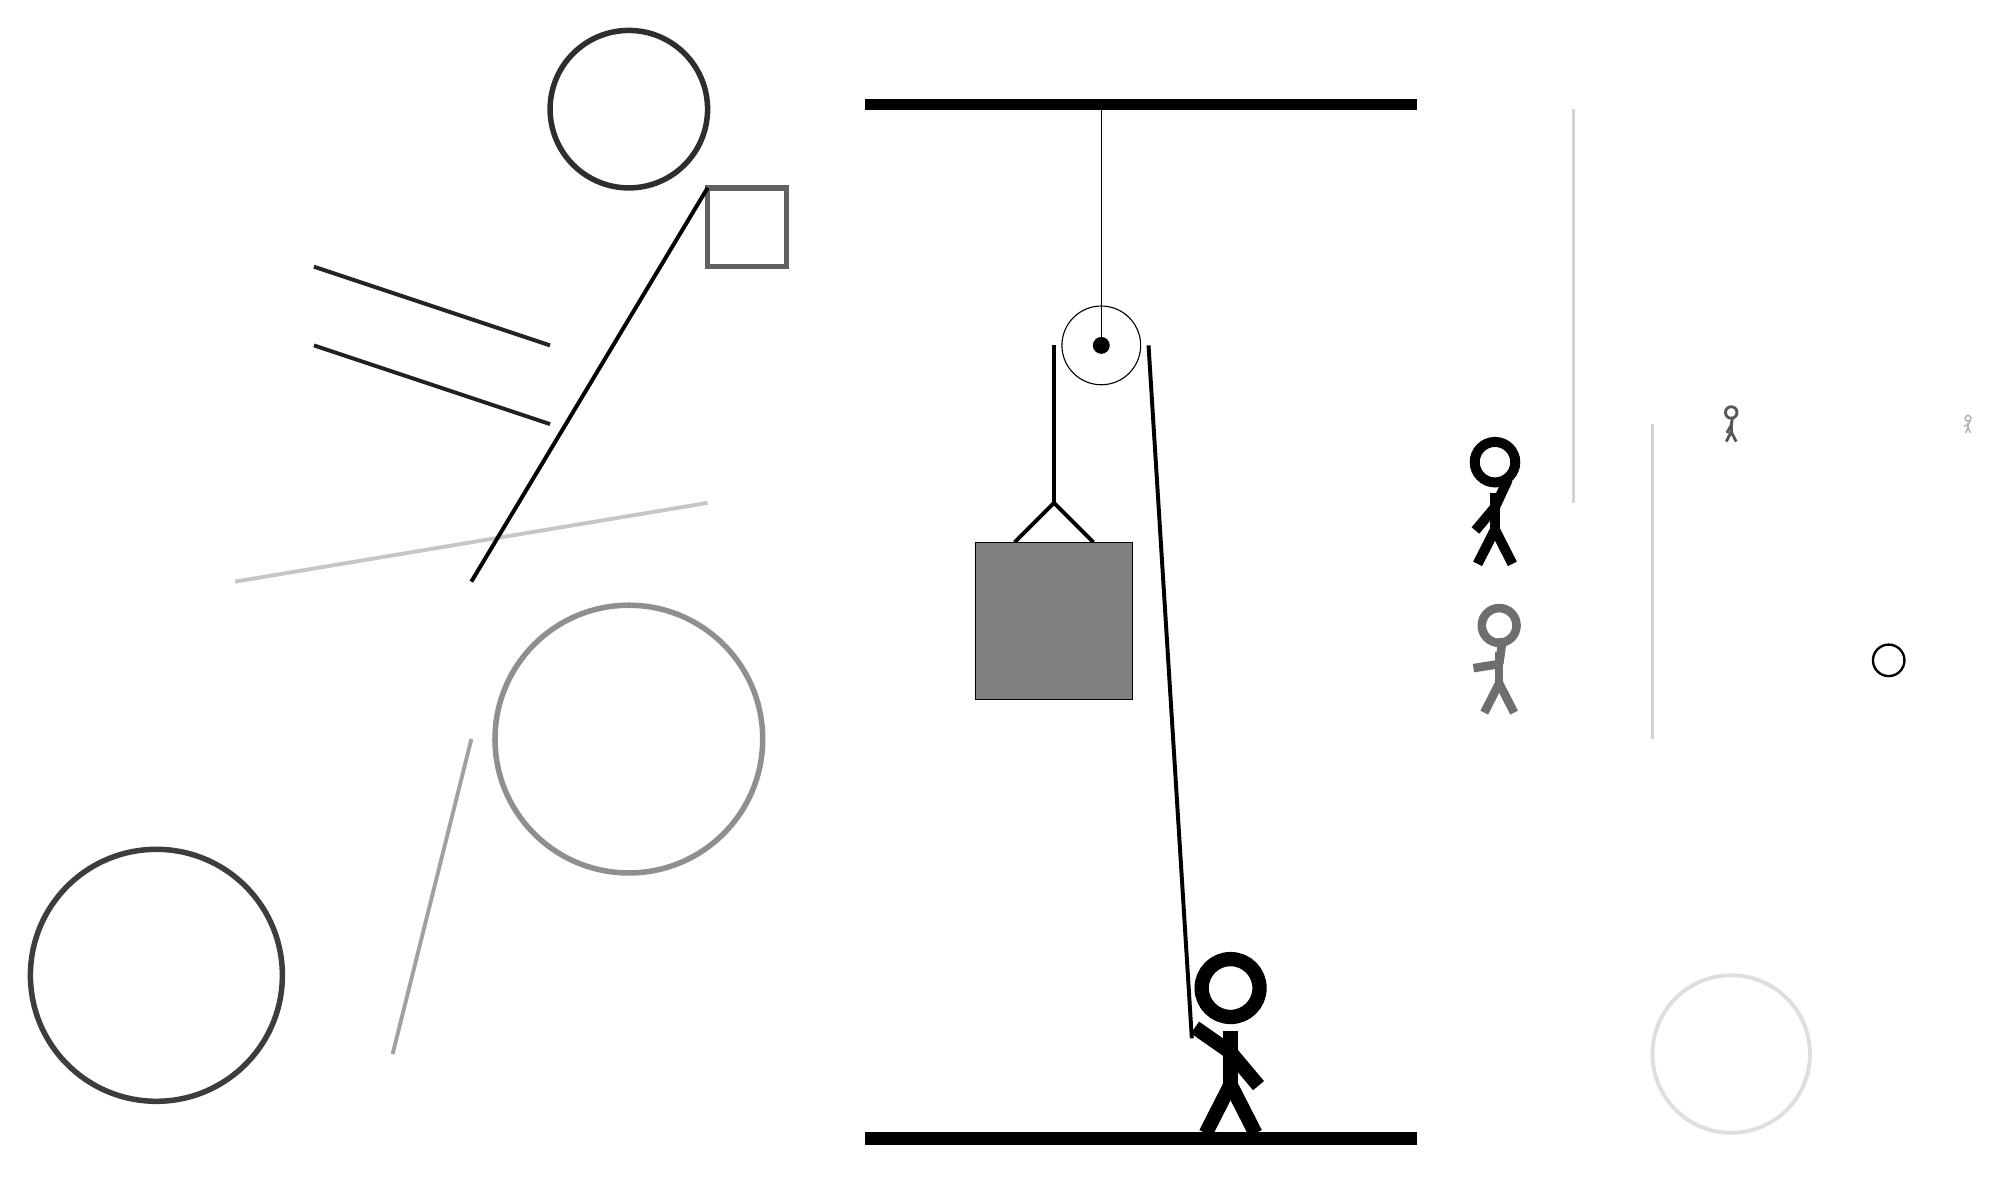
\begin{tikzpicture}
		%%%%% START %%%%%
		
		\draw[fill=black] (-2, 10) rectangle (5, 10.125);
		
		\draw (1, 7) circle (0.5);
		\draw[fill=black] (1, 7) circle (0.1);
		\draw (1, 10) -- (1, 7);
		
		\draw[line width=0.5mm] (-0.1, 4.5) -- (0.4, 5.0) -- (0.9, 4.5);
		\draw[fill=black!50] (-0.6, 4.5) rectangle (1.4, 2.5);
		
		\draw[line width=0.5mm] (0.4, 7) -- (0.4, 5.0);
		\centerarc[line width=0.5mm](1, 7)(0:180:0.6);
		\draw[line width=0.5mm](1.6, 7) -- (2.15, -1.8);
		
		\draw [line width=0.3mm, color=black!99](11, 3) circle (0.2);
		
		\draw [line width=0.5mm, color=black!13](9, -2) circle (1.0);
		\draw[line width=0.5mm, color=black!22](-4, 5) -- (-10, 4);
		\node[line width=0.2mm, color=black!66] at (9, 6) {\Strichmaxerl[2][60][80]};
		\draw[line width=0.5mm, color=black!86](-6, 7) -- (-9, 8);
		
		\draw[line width=0.7mm, color=black!62] (-3, 8) rectangle (-4, 9);
		
		\draw[line width=0.5mm, color=black!87](-6, 6) -- (-9, 7);
		\node[line width=0.7mm, color=black!99] at (6, 5) {\Strichmaxerl[7][50][65]};
		\node[line width=0.3mm, color=black!31] at (12, 6) {\Strichmaxerl[1][21][57]};
		\node[line width=0.3mm, color=black!57] at (6, 3) {\Strichmaxerl[6][9][82]};
		\draw[line width=0.4mm, color=black!17] (7, 5) rectangle (7, 10);
		\draw [line width=0.7mm, color=black!82](-5, 10) circle (1.0);
		\draw [line width=0.7mm, color=black!76](-11, -1) circle (1.6);
		\draw[line width=0.5mm, color=black!100](-7, 4) -- (-4, 9);
		\draw[line width=0.5mm, color=black!37](-7, 2) -- (-8, -2);
		\draw [line width=0.7mm, color=black!44](-5, 2) circle (1.7);
		
		\draw[line width=0.5mm, color=black!18](8, 2) -- (8, 6);
		
		\node at (2.6, -1.9) {\Strichmaxerl[10][-35][-50]};
		
		\draw[fill=black] (-2, -3) rectangle (5, -3.15);
		
		%%%%% END %%%%%
	\end{tikzpicture}
\end{document}